\documentclass[runningheads]{llncs}
\usepackage{graphicx}

\begin{document}
%
\title{Penguin Object Detection Model}

\author{Xunyi Zhao}
\institute{University of Tasmania, Newnham TAS 7248, AU}
\authorrunning{X.}
%
\maketitle
%
\begin{abstract}
Penguin, a near threatened species lives in the southern hemisphere, has been influenced due to the global warming issue recently. The aims of this project is to develop an object detection model, which can  detect and classify the type of penguin from images/videos to help Antarctic scientific research. In this project, popular approaches such as YOLO, Faster R-CNN are used to achieve good performance. On avarage, the AP50 can reach 87\% with the FPS of 161 by using YOLOv7 model, which is 1.5x times faster and +6.3\% AP more accurate than YOLOv5 and even more than Faster R-CNN.

\keywords{Antarctica penguins \and Deep learning \and Object detection \and YOLO \and Faster R-CNN \and Model selection.}
\end{abstract}
%
%

% Section 1: Motivation/real-life benefits
\section{Motivation/real-life benefits}
Penguins, a group of aquatic flightless birds, live almost exclusively in the Southern Hemisphere in Antarctica. Among the 20 living species, the \textbf{\textit{Aptenodytes Forsteri (Emperor Penguin)}}, \textbf{\textit{Aptenodytes Patagonicus (King Penguin)}} and \textbf{\textit{Pygoscelis Antarciticus (Chinstrap Penguin)}} are three of the most common and popular species. 

However, due to the global warming and other issues, emperor penguins have already been identified as Vulnerable or Near Threatened in the lastest IUCN Red List~\cite{ref_red_list}. Sometimes, we may find one or two penguins are isolated on a floating ice (can't find continent or suitable are for living within 10 kilometres around it).

Thus, to help researchers detect this situation, and potentially help them to classify the species of the penguins automatically, or count the number of penguins in the specific area, I selected this project and wish to develop an appropriate deep learning application.

In real life scenario, this application can detect and then identify the species (only from emperor penguins, king penguins and chinstrap penguins due to the time restriction) of penguins live in Antarctica, and count the number of penguins potentially in real-time. What's more, if only one or two penguins are detected within a big area, the system that embedded with this model can send notification, which allows human noticing this situation quickly and providing corresponding aid if necessary. This will benefit both penguin (ensure population ecological balance) and human (needn't monitor manually) a lot.

% Section 2: Data collecting
\section{Data collecting}
In this project, nearly all of the data is collected from Google Image~\cite{ref_google_image}. To ensure the quality of the data and helps the model achieve good performance, I have filtered the bad images manually, for example, images with too many penguins, blurry images, low-resolution images etc.

What's more, since the purpose of the application is to detect and then identify the species (and count the number potentially), it's important for me to collect the images that contains different numbers of penguins (only 1 penguin or many penguins), clear to see (the higher resolution, the better), and in various context and scenario. Besides, the number of samples and penguin instances should also be large enough, and both penguin adults and chicks (they look pretty different) should be included in the data set. To ensure the quality of the data collecting process, if any situation in the following list happens, then I will not collect that image:

\begin{itemize}
  \item If the image size is too small.
  \item If the image ratio is too weird (say 16:3, which means it's not very square).
  \item If the image contains too many penguins (> 100) or blurry.
  \item If the penguins is drawn by human.
\end{itemize}

If the image resolution (size) is low, the image will be even more blurry after resizing before/during the training process, so that the model could not extract the key features of the image and the performance will be impacted. Also, if the image is too narrow (strange image ratio), then the object will be squeezed/stretched too much after resizing, causing difficulties for model to recognized these objects. All this aspects will be discussed again in the model selection part.

Another step in data collecting is the data augmentation. Augmentation performs transforms on the existing images to create new variations and increase the number of images in the data set. This ultimately makes models more accurate across a broader range of use cases. 
In the real scenario, the environment we monitor may contain some noise and the exposure of the photo/video of the observed environment will be different, which would affect the average precision of the model. To help the model be more resilient to camera artifacts, lighting and camera setting changes, I choose to generate more pictures with different \textbf{noise} (Up to 3\% of pixels) and \textbf{exposure} (Between -15\% and +15\%) using Roboflow tool~\cite{ref_roboflow}


% Section 3: Data annotating
\section{Data annotating}
To annotate the data that I've collected, I also used Roboflow~\cite{ref_roboflow}. Each types of penguins can be labeled using bounding box with different colors within a short time. 
The following are the rules I stick with to ensure the quality of the data annotating process:
\begin{itemize}
  \item Make sure the bounding box cover the whole body of each penguin.
  \item If the image contains many penguins, and some of the penguins are too small/blurry/not distinctly visible, just annotate the clear penguins that stand in the front.
  \item If only the head of the penguin can be seen, make sure to annotate the head.
  \item Annotate the penguin chick as well.
\end{itemize}
The reason why I ignored some penguins that are too small/blurry/not distinctly visible is that, although as human, we can know that these "objects" are emperor penguins or king penguins, but if the model learns many of these "information", it would have some problems such as over-fitting or can't detect the penguins correctly (treat any similar blurry things as penguin which is not good for general case). However, it doesn't mean computer couldn't detect the blurry penguins since computer vision is in pixel-level but human is not . If the application is used for counting the number of penguins in the image, then I should label all the penguins that I can see.
But the main purpose is to detect and classify, to balance this situation, I choose to ignore the blurry penguins in the background.

% Section 4: Data processing
\section{Data processing}
Data preprocessing is a crucial phase in the machine learning process since the quality of the data and the information that can be extracted from it directly influence how well our model can learn. For this reason, it is crucial that we preprocess the data before introducing it to the model.

Since the images I collected don't have the same size (resolution), although in some models like YOLOv5 the image resizing is done automatically, it's still a good practice to resize the image into same size (the reason will be discussed in the later <b>Model Evaluation and Selection</b> section). Thus, to help the model learn better, the Resize option should be chosen as such: 

Usually, an image is captured with metadata that specifies how it should be displayed in relation to how the pixels are arranged on disc. This directive, which is stored in the EXIF orientation field, expedites the image encoding process at the time of capture, allowing cameras to efficiently sample data from their sensors without unwelcome artefacts.

This means that most cameras store images' pixels exactly the same whether the camera is oriented in landscape or portrait mode. They just flip a bit to signal to the viewer whether to display the pixels as-is or to rotate them by 90 or 180 degrees when displaying the image.

Unfortunately, this can cause issues if the application displaying the images is unaware of the metadata and naively displays the image without respecting its EXIF orientation. Thus, to help the model learn better, the Auto-Orient option should always be chosen as such: 

During the data annotating, I used the scientific name for each type of penguin which is hard for general user to understand. Thus, to help user know what the species are when the model detecting objects, the Modify classes option should be chosen as such:

\subsubsection{Sample Heading (Third Level)} Only two levels of
headings should be numbered. Lower level headings remain unnumbered;
they are formatted as run-in headings.

\paragraph{Sample Heading (Fourth Level)}
The contribution should contain no more than four levels of
headings. Table~\ref{tab1} gives a summary of all heading levels.

\begin{table}
\caption{Table captions should be placed above the
tables.}\label{tab1}
\begin{tabular}{|l|l|l|}
\hline
Heading level &  Example & Font size and style\\
\hline
Title (centered) &  {\Large\bfseries Lecture Notes} & 14 point, bold\\
1st-level heading &  {\large\bfseries 1 Introduction} & 12 point, bold\\
2nd-level heading & {\bfseries 2.1 Printing Area} & 10 point, bold\\
3rd-level heading & {\bfseries Run-in Heading in Bold.} Text follows & 10 point, bold\\
4th-level heading & {\itshape Lowest Level Heading.} Text follows & 10 point, italic\\
\hline
\end{tabular}
\end{table}


\noindent Displayed equations are centered and set on a separate
line.
\begin{equation}
x + y = z
\end{equation}
Please try to avoid rasterized images for line-art diagrams and
schemas. Whenever possible, use vector graphics instead (see
Fig.~\ref{fig1}).

\begin{figure}
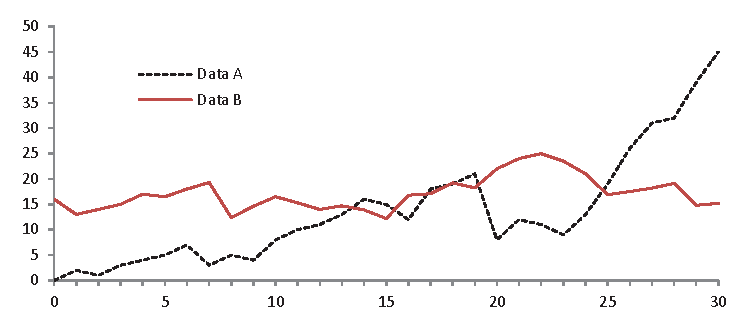
\includegraphics[width=\textwidth]{fig1.eps}
\caption{A figure caption is always placed below the illustration.
Please note that short captions are centered, while long ones are
justified by the macro package automatically.} \label{fig1}
\end{figure}

\begin{theorem}
This is a sample theorem. The run-in heading is set in bold, while
the following text appears in italics. Definitions, lemmas,
propositions, and corollaries are styled the same way.
\end{theorem}

% Section 5:
\section{Model selection/design}

% Section 6:
\section{Model selection}
\subsection{Selection strategy and metrics used}
\subsection{Results analysis}
\subsection{Select the best model}
% Section 6:
\section{Apply the model}
% Section 8:
\section{Post-analysis}
\subsection{Advantages/disadvantages of the approaches}
\subsection{Potential improvement}
\subsection{Other models/approaches}


% Reference
\begin{thebibliography}{8}
\bibitem{ref_red_list}
IUCN 2021, The IUCN Red List of Threatened Species, IUCN Red List of Threatened Species, IUCN.

\bibitem{ref_google_image}
Google Images n.d., Google.com.

\bibitem{ref_roboflow}
Roboflow: Go from Raw Images to a Trained Computer Vision Model in Minutes. n.d., roboflow.ai.

\end{thebibliography}
\end{document}
